\renewcommand{\SS}{\mathbb{S}}
\newcommand{\Par}[2]{\mbox{$( #1, #2 )$}}
\usetikzlibrary{positioning, shapes, trees, graphs} % RNA trees
\newcommand{\scale}{0.6}

\newcommand{\tree}[1]{\ensuremath{#1}}

\chapter{Uvod do študia štruktúry RNA a grafov}
Na začiatku práce stručne zoznámime čitateľa s pojmamy, ktoré s RNA a jej štruktúrou súvisia.


\section{Co je RNA}

% TODO pridat nejaky vseobecny uvod, napriklad, ze RNA hraje velku ulohu pri prepise genetickej informacie a pod. potom veta ze je jednovlaknova a ze to vlakno sa sklada z molekul z 3 zloziek - cukor, fosfat a dusikata baza. Potom ze my dalej budeme na vsetko ostatne kaslat a stavebnou jednotkou bude pre nas prave baza A C G U.
 
 Ribonukleónová kyselina je nukleonová kyselina tvorená jedným vláknom kovalentne naviazaných ribonukleotidov, 
 ktoré sú základnými stavebnými jendotkami nukleonových kyselín. Je biochemicky odlišná od DNA kôli prítomnosti 
 hydroxilovej skupiny pripojenej ku každej molekule pentózy v reťazci.
 v DNA a RNA sa vyskytuje niekoľko variant nukleotidov (báz). U RNA sú to
adeín (A), guanín (G), cytozín (C), uracyl (U),
pri DNA sa namiesto uracylu vyskytuje tymin (T).
Medzi jednotlivými bázami sa môžu vyskytovať vodíkové väzby. Nukleotidy majú
vzájomnú preferenciu, čo znamená, že bázy vznikajú najčastejšie medzi A-U a C-G
u RNA a podobne A-T a C-G u DNA.

Štrukturu nukleových kyselín môžeme chápat podľa stupňa zjednodušenia
\begin{itemize}
  \item Primárna štruktúra - je určená poradím jednotlivých nukleotidov
    do polynukleotidového reťazca
  \item Sekundárna štruktúra - je daná parovaním medzi bázami molekuly
  \item Terciárna štruktúra - priestorové usporiadanie molekuly
\end{itemize}
DNA je dvojvláknova molekula, u ktorej spojenie medzi vlaknami sa realizuje na princípe
komplementarity.
Naopak, RNA je iba jednovláknova molekula a v snahe minimalizovať voľnu energiu molekuly,
sa paruje sama na seba. V tomto hrajú rolu pritazlive sily medzi bázami.

V praci budeme štruktúrou myslieť práve sekundárnu štruktuúru RNA, ak nebude povedané inak.

Až donedávna sa myslelo, že funkcia RNA je obmedzená na prenos genetickej informácie z DNA
v jadre bunky do ribozomu. Napríklad pri tvorbe bielkovín (mRNA), alebo transporter aminokyselin
v ribozome bunky (tRNA).
% TODO: citacie k druhom RNA
Avšak existuje mnoho ďalších, od relatívne
malých molekúl tvorenyých desiatkami báz, ktoré pomáhajú pri expresii genov
(miRNA, siRNA, tmRNA a dalsie), až po veľké, tvorené tisíckami nukleotidov (rRNA).

\section{Sekundarna struktura rRNA + konzervovanost}

Ako hlavný objekt záujmu sme si spomedzi všetkych druhov RNA vybrali práve ribozomálnu,
najmä kvôli jej veľkosti a tomu, že existujúcim nástrojom práve veľkosť robí najväčšie problémy
pri vizualizácii.

\begin{definice}[Primárna štruktra RNA]
  \label{def:RNA_primarna_struktura}
  Nech $\Sigma$ je abeceda $\{A, C, G, U\}$. Potom slovo $W \in \Sigma^n$ nad touto abecedou
  je sekvencia nukleotidov (baz) RNA.
\end{definice}

Jednotlivé nukleotidy sekvencie RNA budeme, ak bude zretelné o čo sa jedná, označovat priamo poradovým 
číslom, teda $i$ bude označovať nukleotid $W_{i}$, resp. $W[i]$.

\begin{definice}[Sekundarna struktura RNA]
  \label{def:RNA_sekundarna_struktura}
  Nech $W$ je sekvencia podla definicie \ref{def:RNA_primarna_struktura} dlzky n.
  Sekundarnou strukturou oznacime mnozinu $\SS$ parov nukleotidov \Par{i}{j} takych, ze
  pre dva pary \Par{i}{j} a \Par{k}{l} $\in \SS$ (bez ujmy na obecnosti $i \leq k$)
  plati jedno z nasledujucich:
  \begin{itemize}
    \item $i = k \iff j = l$
    \item $i < j < k < l$, cize par \Par{i}{j} predchadza par \Par{k}{l}
    \item $i < k < l < j$, cize par \Par{i}{j} obsahuje par \Par{k}{l}
  \end{itemize}
\end{definice}

%TODO: obrazok prim/sek/terc struktury RNA

Prvá podmienka zabezpečuje, že nukleotid je najviac v jednom bazickom páre, druhá a tretia
hovoria o usporiadani párov, buď sú na sebe nezávisle alebo na seba nadväzujú.
Posledna podmienka zakazuje existenciu pseudouzlov (pseudoknots). Pseudouzol patrí medzi najčastejšie typy priestorového usporiadania RNA. Vytvára  niekolko interakcii vrámci jednej molekuly a smyčky typu loops,  ktore vznikajú medzi rôznimy molekulami.

%TODO: pseudoknot obrazok
%TODO: 2 obrazky RNA napriec fylogenetickym stromom

\begin{figure}[H]
\centering
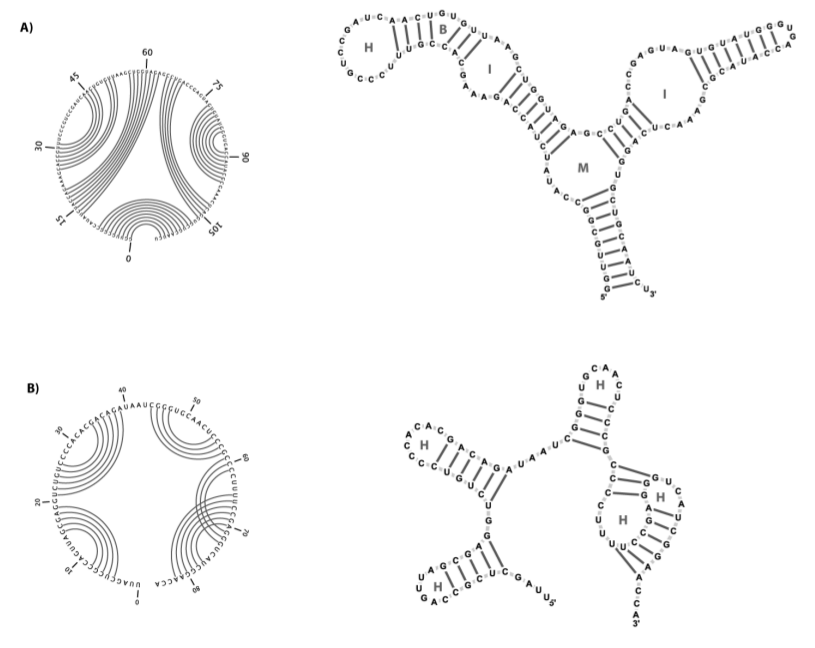
\includegraphics[width=140mm, height=120mm]{../img/RNA_circular_reprezentation.png}
\caption{Circular Feynman - kruhova reprezentacia sekundarnej struktury}
\label{obr:RNA_circular_representation}
\end{figure}


\subsection{Motivy}

Motivom v RNA máme na mysli časti molekuly, ktoré vytvárajú určité štruktúry.
Na obrazku \ref{obr:RNA_motifs} vidime motivy, ktore sa mozu v RNA vyskytovat.

Stem (stonka) je časť molekuly kde sa na seba paruju dva súvisle časti RNA vlákna.
Interior loop spája dva stemy a medzi nimi na oboch stranách obsahuje nespárované
bázy. Podobna je bulge (vypuklina), ale nespárované nukleotidy ma iba z jednej strany.
Hairpin je medzi časťami vlákna, ktoré sa parujú sami na seba.
Multibranch loop je podobná ako interior loop, ale spája dokopy viac stemov.
V ďalšom rozprávani ámam bude stačiť rozdelenie na stem a loop.

%TODO: ako nazyvat strukturne motivy v RNA: anglicky, alebo hladat vhodny preklad

\begin{figure}[H]
\centering
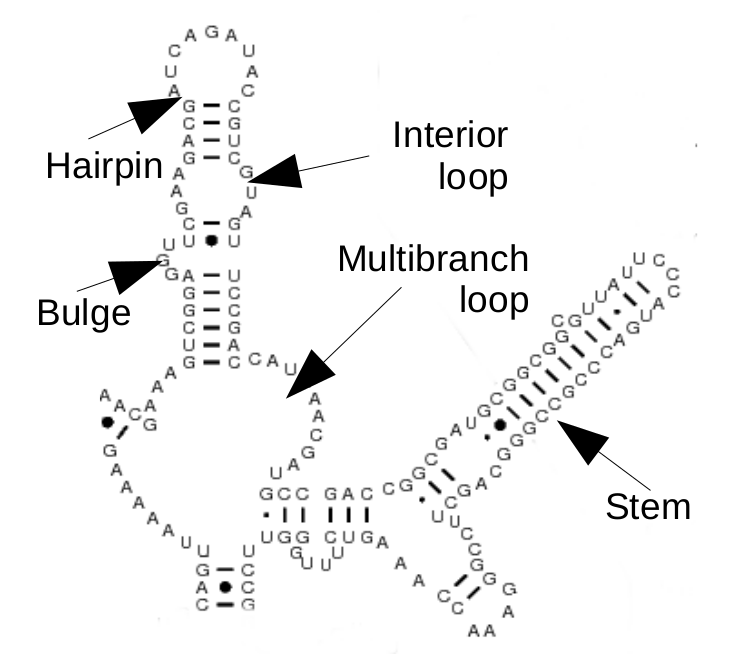
\includegraphics[width=70mm, height=70mm]{../img/struktury_v_rna.png}
\caption{Strukturalne motivy v RNA}
\label{obr:RNA_motifs}
\end{figure}

\section{Grafové pojmy}

Potrebujeme si definovať značenie a pojmy, ktoré budeme používať naprieč celou prácou.
Z väčšej časti použijeme značenie od \citet{RTED}.

\subsection{Značenie}

\begin{definice}\label{def:strom}
  Usporiadaný zakorenený strom je orientovaný graf, v ktorom platí, že v ňom neexistujú cykly
  a že hrany sú orientované vždy v smere z predka na potomka.
  Okrem koreňa má každý vrchol svojho predka. Naviac tu existuje usporiadanie medzi potomkami.
  \\
  Usporiadany les je usporiadaná množina stromov.
  %TODO: obrázok usporiadania stromov
\end{definice}

Ak \tree{F} je les, $V_F$ budeme označovať množinu jeho vrcholov a $E_F$ množinu jeho hrán.
Prázdny strom/les budeme značiť $\emptyset$.

Podles lesa \tree{F} je les \tree{G} s vrcholmi $V_{\tree{G}} \subseteq V_{\tree{F}}$
a hranami $E_{\tree{G}} \subseteq E_{\tree{F}} \cap (V_{\tree{G}} \times V_{\tree{G}})$.
Obdobne to plati aj pre podstrom stromu.

Nech $v$ je vrchol stromu \tree{F}. Potom \tree{F_{v}} budeme značiť podstrom \tree{F} zakorenený vo $v$,
t.j. v strome ostávajú iba potomkovia $v$.
\\
\tree{F - v} budeme značiť les, ktorý vznikne zmazaním vrcholu $v$ z \tree{F} spolu so
všetkými hranami obsahujúcimi $v$. Podobne \tree{F - \tree{F_{v}}} budeme značiť les, ktorý
dostaneme zmazaním podstromu \tree{F_{v}} z \tree{F}.

\begin{definice}
  Nech \tree{F} je strom, $u$ a $v$ jeho dva rôzne vrcholy.
  Hovoríme, že $u$ je predkom $v$ ($v$ je potomok $u$) ak $(u, v) \in E_{\tree{F}}$.
  Hovoríme, že $u$ je súrodencom $v$, ak sú to rôzne vrcholy a majú spoločného predka.
\end{definice}



\section{Stromová reprezentacia sekundarnej struktury}

Definicia \ref{def:RNA_sekundarna_struktura} nám ponúka reprezentovať sekundárnu štrukturu
ako usporiadaný strom.

\begin{figure}[H]
\centering
%TODO: vlastny obrazok... namiesto clankoveho
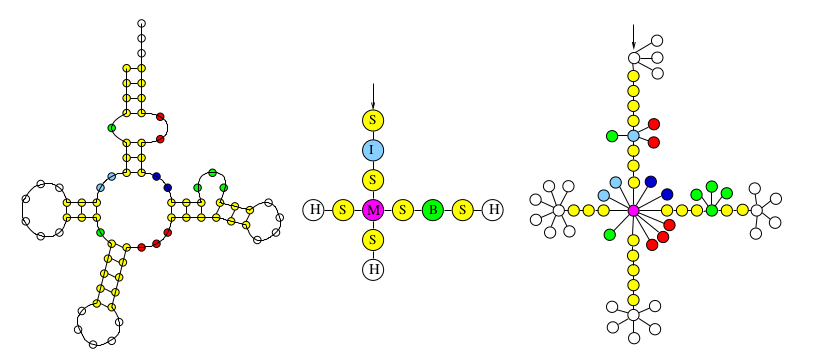
\includegraphics[width=130mm, height=70mm]{../img/stromova_reprezentacia_rna.png}
\caption{Varianty reprezentacie vrcholov}
\label{obr:RNA_vrcholy}
\end{figure}

Bez ujmy na obecnosti budeme o RNA hovoriť ako o strome, aj keď sa môže stať, že
štruktúra nebude celistvá (teda nieje to strom, ale les). V tom prípade ale
iba pripojíme koreňový vrchol, ktorého potomkovia budú dané stromy.

Každý vrchol stromu môže reprezentovať napríklad motiv v štruktúre RNA, nukleotid, alebo bázovy pár
Príklady možno vidiet na obrázku \ref{obr:RNA_vrcholy}.

V našej práci vrchol stromu reprezentuje bázovy pár (vnútorný vrchol) a nespárovanú bázu (list stromu).
Štruktúru, do ktorej patrí si totiž vieme ľahko zistiť z potomkov vrcholu.

%rna, from 5' to 3':
% AUGCAAACUGGCACCCUCAU
% (((((...))(...))..))

\begin{center}
  \begin{minipage}{.500\textwidth}
    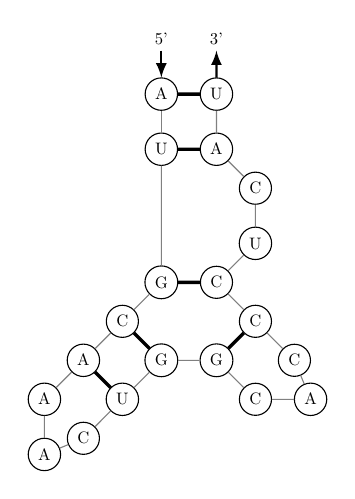
\begin{tikzpicture}[
        on grid,
        node distance = 0.7,
        -latex,
        scale = \scale,
        every node/.style = {scale = \scale},
        base/.style = {circle, draw},
        ends/.style = {draw = none, fill = none}]

      %ends, 5' a 3'
      \node[ends] (5end) {5'};
      \node[ends] (3end) [right = of 5end] {3'};

      %stem
      \node[base] (StemLeft1) [below = of 5end] {A};
      \node[base] (StemRight1) [right = of StemLeft1] {U};
      \node[base] (StemLeft2) [below = of StemLeft1] {U};
      \node[base] (StemRight2) [right = of StemLeft2] {A};

      %bulge
      \node[base] (Bulge1) [below right = of StemRight2] {C};
      \node[base] (Bulge2) [below = of Bulge1] {U};

      %stem
      \node[base] (StemRight3) [below left = of Bulge2] {C};
      \node[base] (StemLeft3) [left = of StemRight3] {G};

      %left-branch
      \node[base] (LBranchLStem1) [below left = of StemLeft3] {C};
      \node[base] (LBranchRStem1) [below right = of LBranchLStem1] {G};
      \node[base] (LBranchLStem2) [below left = of LBranchLStem1] {A};
      \node[base] (LBranchRStem2) [below left = of LBranchRStem1] {U};

      %left-branch-hairpin
      \node[base] (LBranchHairpin1) [below left = of LBranchLStem2] {A};
      \node[base] (LBranchHairpin2) [below = of LBranchHairpin1] {A};
      \node[base] (LBranchHairpin3) [below left = of LBranchRStem2] {C};

      %right-branch
      \node[base] (RBranchRStem1) [below right = of StemRight3] {C};
      \node[base] (RBranchLStem1) [below left = of RBranchRStem1] {G};

      %right-branch-hairpin
      \node[base] (RBranchHairpin1) [below right = of RBranchLStem1] {C};
      \node[base] (RBranchHairpin2) [right = of RBranchHairpin1] {A};
      \node[base] (RBranchHairpin3) [below right = of RBranchRStem1] {C};

      \begin{scope}[-]
      %pair edges
        \path[very thick]
        (StemLeft1) edge (StemRight1)
        (StemLeft2) edge (StemRight2)
        (StemLeft3) edge (StemRight3)
        (LBranchLStem1) edge (LBranchRStem1)
        (LBranchLStem2) edge (LBranchRStem2)
        (RBranchLStem1) edge (RBranchRStem1)
        ;
      %lines around molecule
        \path[color = gray]
        (StemLeft1) edge (StemLeft2)
        (StemLeft2) edge (StemLeft3)
        (StemLeft3) edge (LBranchLStem1)
        (LBranchLStem1) edge (LBranchLStem2)
        (LBranchLStem2) edge (LBranchHairpin1)
        (LBranchHairpin1) edge (LBranchHairpin2)
        (LBranchHairpin2) edge (LBranchHairpin3)
        (LBranchHairpin3) edge (LBranchRStem2)
        (LBranchRStem2) edge (LBranchRStem1)
        (LBranchRStem1) edge (RBranchLStem1)
        (RBranchLStem1) edge (RBranchHairpin1)
        (RBranchHairpin1) edge (RBranchHairpin2)
        (RBranchHairpin2) edge (RBranchHairpin3)
        (RBranchHairpin3) edge (RBranchRStem1)
        (RBranchRStem1) edge (StemRight3)
        (StemRight3) edge (Bulge2)
        (Bulge2) edge (Bulge1)
        (Bulge1) edge (StemRight2)
        (StemRight2) edge (StemRight1)
        ;
      \end{scope}

      \begin{scope}
        % edges to ends
        \path[thick]
        (5end) edge (StemLeft1)
        (StemRight1) edge (3end)
        ;
      \end{scope}
    \end{tikzpicture}
  \end{minipage}
  \begin{minipage}{.450\textwidth}
    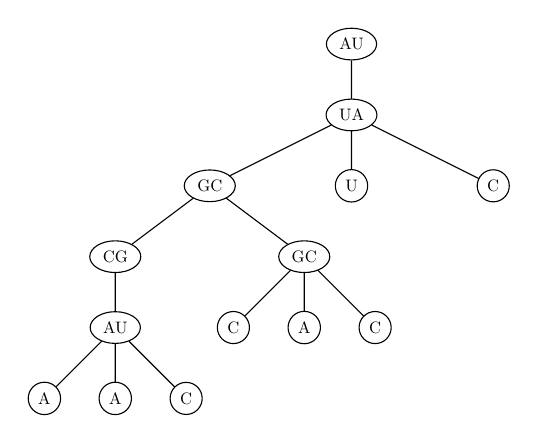
\begin{tikzpicture}[
        baseline,
        level distance = 1.5 cm,
        scale = \scale,
        every node/.style = {scale = \scale},
        basepair/.style = {ellipse, draw, minimum height = 0.3 cm, minimum width = 0.7 cm},
        unpaired/.style = {circle, draw, minimum width = 0.3 cm},
        level 2/.style = {sibling distance = 3 cm},
        level 3/.style = {sibling distance = 4 cm},
        level 4/.style = {sibling distance = 1.5 cm}
      ]
      \node[basepair] {AU}
      child {
        node[basepair] {UA}
        child {
          node[basepair] {GC}
          child {
            node[basepair] {CG}
            child {
              node[basepair] {AU}
              child {
                node[unpaired] {A}
              }
              child {
                node[unpaired] {A}
              }
              child {
                node[unpaired] {C}
              }
            }
          }
          child {
            node[basepair] {GC}
            child {
              node[unpaired] {C}
            }
            child {
              node[unpaired] {A}
            }
            child {
              node[unpaired] {C}
            }
          }
        }
        child {
          node[unpaired] {U}
        }
        child {
          node[unpaired] {C}
        }
      }
      ;
    \end{tikzpicture}
      %\caption{Stromova reprezentacia RNA}
      %\label{obr:RNA_tree}
  \end{minipage}
\end{center}





